\chapter{Обзор современного состояния бортовых оптико-электронных систем специального назначения} \label{ch:ch1}

В современных условиях применения в предполагаемых локальных и региональных военных конфликтах обычного вооружения важнейшую роль играют  \hyperref[acroLA]{ЛА} тактической военной авиации, например: самолеты, вертолеты и беспилотные летательные аппараты (\hyperref[acroUAV]{БЛА}). Они являются одним из основных средств борьбы с предполагаемым наземным, надводным и воздушным противником. При этом существенным требованием является выполнение ими предполагаемых боевых действий круглосуточно, в простых и сложных метеоусловиях. 

Одним из основных компонентов бортового радиоэлектронного оборудования вышеуказанных  \hyperref[acroLA]{ЛА} являются оптико-электронные обзорно-поисковые 
(рисунок \ref{fig:soep}) и прицельные системы, обеспечивающие более высокую точность по сравнению с радиолокационными системами, особенно при работе по малоразмерным целям. В свою очередь, пилотажные \hyperref[acroEOS]{ОЭС} обеспечивают маловысотное пилотирования \hyperref[acroLA]{ЛА} к району ведения боевых действий с обходом находящихся по курсу полета препятствий с целью снижения своей видимости радиолокационными средствами  \hyperref[acroPVO]{ПВО}.

\begin{figure}[ht]
	\centering
 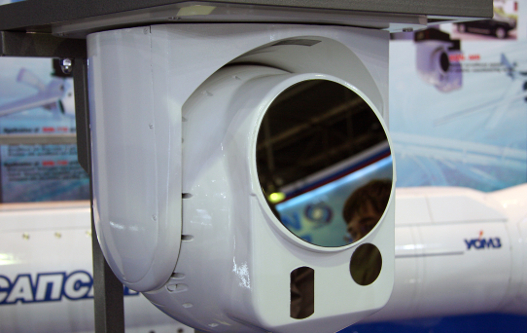
\includegraphics[width=0.5\linewidth]{p1} 
 \caption{Оптико-электронная система СОН-730}
 \label{fig:soep}
\end{figure}

Радикальным преимуществом \hyperref[acroEOS]{ОЭС} по сравнению с радиолокационными является также и гораздо более высокая скрытность их работы, что существенно повышает выживаемость  \hyperref[acroLA]{ЛА} в ходе проведения ими боевых действий. 

Однако у этих систем есть большой недостаток по сравнению с радиолокационными существенная зависимость их рабочих характеристик от метеоусловий и невозможность работы через облачность в видимой области спектра. 

По реализуемым ТТХ многие отечественные авиационные  \hyperref[acroEOS]{ОЭС}, к сожалению, отстают от современного мирового уровня. Это обусловлено, главным образом, более низким качеством отечественной оптико-электронной элементной базы для них и технологического производственного оборудования. Одним из важных факторов достижения успешного конкурентоспособного результата является применение строгих методик разработки и исследования динамики вновь разрабатываемых или модернизируемых САУ \hyperref[acroAEOS]{БОЭП}, использование информационных технологий для ускорения разработки изделий и уменьшения количества ошибок. Отсутствие процесса моделирования системы управления во время разработки прибора так же может снижать общую надежность и конкурентоспособность изделия.

%Крайне важно видеть наиболее перспективные направления совершенствования отечественной оптико-электронной техники выбирая наиболее перспективные направления как по степени их приоритетности, так и по минимуму технических рисков. 

В этой связи для разработчиков и потребителей отечественных  \hyperref[acroLA]{ЛА} значительный интерес представляют данные по серийным авиационным оптико-электронным системам, используемым в настоящее время в зарубежной авиационной практике. Одновременно для них представляют интерес и тенденции совершенствования этих систем для понимания в каких направлениях целесообразно продвигаться дальше. 

Целью данного обзора является представление информации по этим вопросам, а также сравнительный анализ представленных систем по критерию выполняемой боевой задачи. 

Обзор современного состояния \hyperref[acroEOS]{ОЭС} специального назначения проведен по следующим направлениям:
\begin{enumerate}
	\item Обзорно-поисковые, прицельные и пилотажные оптико-электронные системы;
	\item Авиационные \hyperref[acroEOS]{ОЭС} инфракрасного противодействия ракетной атаке;
	\item Анализ элементной базы обеспечения обратной связи в современных  \hyperref[acroEOS]{ОЭС};
	\item Математические модели, динамика и управление, синтез и компьютерное моделирование САУ бортовых ОЭС.
\end{enumerate}

\section{Обзорно-поисковые оптико-электронные системы} \label{sec:ch1/sec1-}

Для изучения проблем и задач создания  \hyperref[acroEOS]{ОЭС} смотрящего типа базирующейся на  \hyperref[acroLA]{ЛА}, рассмотрим некоторые аналогичные приборы зарубежного и Российского производства. Таблица \ref{tab:EOS} демонстрирует зарубежные и российские авиационные обзорно-поисковые, следящие оптико-электронные системы, за последние 10 лет. 

\begin{landscape}

\begin{longtable}{| p{6cm} | p{18cm} |}
	\caption{Поисково-следящие системы авиационного базирования}%
	\label{tab:EOS}% label всегда желательно идти после caption
	\\ \hline
		Название комплекса, 
		
		Страна производитель, 
		
		Год начала производства, 
		
		Масса 
		& 
		Назначение, Области применения, Принципы построения, Технические хар-ки, Технологии, Конструктивные особенности, Перспективы развития 
	\\ \hline
		OSF (Optronique Secteur Frontal). Thales Optronics, SAGEM, \cite[]{OSF}
		
		Франция, 
		
		2010 г., 
		
		95 кг. 
	& 
		\small 3-5 + 8-12 мкм-IRST, ЛД-1,54. Установлена в верхней носовой части самолета перед кабиной фюзеляжа выведены 2 раздельные IRST- и ДТВ + ЛД-головки. Последняя является ОМБ ОП-подсистемы "CIU" (Combat Identification Unit), предназначенной как для наведения на воздушные цели УР "воздух-воздух", так и для решения прицельных задач по земле, воде. 
	    \small IRST-подсистема обеспечивает круглосуточное обнаружение и распознавание воздушных целей, имеет ТпВ-режим. Фотоматериал и топология используемых в ней фоточувствительных элементов не сообщаются (по косвенным данным, в обоих диапазонах используются сканирующие 4х288 эл.-субматрицы). 
		
		
		\small Днем для более точного распознавания и идентификации этих целей используется узкопольный ДТВ из состава ОП-подсистемы "CIU". Со временем планируется заменить его на круглосуточную ТВ-камеру. По имеющимся данным, дальность обнаружения воздушных целей IRST-подсистемой составляет Rо 80...100 км, ДТВ 30...50 км, типовых наземных целей соответственно 40 (в ТпВ-режиме) и 35 км. 
		
		\small Основную же нагрузку при решении ударных задач по земле, воде несет уже приводившаяся ранее, также предназначенная для использования на самолете Rafale контейнерная ОПС "DAMOCLES".
	\\ \hline
		IR OTIS. Saab Bofors Dynamics \cite[]{doi:10.1117/12.450557},
		
		Швеция	
		
		2010 г,	
		
		30-10 кг
		 
	& 
		\small Встроенная 8-12 мкм-IRST + ОП-система для шведского самолета Jas 39 Gripen.  Данная система предназначена для работы по воздуху и земле. В ней используется сканирующий фотоприемник с числом элементов nэл 1200, фоточувствительный материал и топология расположения элементов не сообщаются (по косвенным данным, это 4х288 эл-КРТ-субматрица). Она может работать как с широкими полями зрения для быстрого обзора, так и с узкими для обнаружения целей на больших дальностях. Опять же по косвенным данным, эти поля равны 12х12 / 5,5х5,5 / 2х2о. 
		\small Сектора обзора могут выставляться оператором в заданных направлениях в пределах передней полусферы самолета. Система может работать в IPST-режиме сразу по многим целям "на проходе" и в ТпВ-режиме осуществлять точное АС выбранной цели. 
		\small ОМБ установлен на верхней носовой части фюзеляжа самолета, перед кабиной, несколько левее строительной оси самолета для обеспечения ограниченного обзора земной поверхности. 
		 
	\\ \hline
		Strix / Nightowl. SAGEM	
		
		Франция	
		
		2000 г. 	
		
		105 кг 
	& 
		\smallДля французского эскортного вертолета Tigre HAP. Надкабинное размещение, также может наводить на цели ПТУР "HOT" и "Hellfire". Оптический визир (ОВ), 3х-польные ДТВ, 8-12 мкм-ТпВ-II, ЛД-1,54, ИК-пеленгатор ПТУР "HOT", может быть ЛДЦ-1,06 / 1,54, ПЛП. Может наводиться на цели от НСЦИ пилота. В ТпВ используется сканирующая 4х288 эл.-КРТ-субматрица, мини ЭЛТ вводит ДТВ- и ТпВ-изображения в окуляр ОВ (возможна модификация и без ОВ). При изготовлении корпуса ОМБ этой ОПС используются облегченные композитные материалы, что крайне важно для надкабинного конструктивного исполнения.
		 
	\\ \hline
		M-TADS / PNVS. Lockheed Martin, DRS Technologies
		\cite[]{lockheedmartin}
		
		США	
		
		2005 г. 
		 
	& 
		\small ОП + пилотажная  \hyperref[acroEOS]{ОЭС} американского армейского вертолета AH-64D Apache Longbow. Носовое размещение. В состав ОП-подсистемы "M-TADS" входят ч/б ДТВ, 3-5 мкм-ТпВ-III, 8-12 мкм-ТпВ-II, ЛДЦ-1,06 / 1,54, ПЛП, ИНС / GPS, в состав пилотажной подсистемы "M-PNVS" широкопольные НУТВ и 8-12 мкм-ТпВ-II. В 8-12 мкм-ТпВ-II-каналах обеих подсистем используются сканирующие 4х480 эл.-КРТ-субматрицы, в 3-5 мкм-ТпВ-III-канале ОП-подсистемы смотрящая 320х256 эл.-InSb-матрица + микроскан (nэл экв= 640х512). Последний размещен в одном отсеке с ДТВ, при этом отсек имеет прозрачное для обоих этих каналов сапфировое входное окно. В обеих подсистемах предусмотрены интегрирование ТВ- и ТпВ-изображений, выдача их на НСЦИ пилотов и, в оцифрованном виде, на землю и на другие  \hyperref[acroLA]{ЛА}.
		 
	\\ \hline
		CоMPASS.		
		
		2001 г. 	
		
		38 - 35 кг 
& 
\small Панкратический ч/б или цветной ДТВ, 3х-польный 3-5 мкм-ТпВ-III, ЛД-1,54 или ЛЦУ-1,06, ПЛП, 0,8 мкм-лазерный маркер. Может быть 8-12 мкм-ТпВ-II. В 3-5 мкм-ТпВ используется 320х256 эл.-InSb-матрица + микроскан (nэлэкв = 640х512), он может быть панкратическим. В 8-12 мкм-ТпВ используются сканирующая 4х288 эл.-КРТ-субматрица и дискретные поля зрения. ЛД-1,54 на Er-стекле, в ЛЦУ-1,06 используется ППЛ-накачка. Его энергия в импульсе Еи 80 мДж, частота повторения Fи 20 Гц. Мощность излучения маркера Ризл 50 мВт. 
 
\\ \hline
		D-CоMPASS.
				
		2005 г. 
			
		32 - 41 кг 
& 
\small Могут быть ч/б или цветной ДТВ, 3-5 мкм-ТпВ-III, 8-12 мкм-ТпВ-II, ЛД-1,54, ЛДЦ-1,06 / 1,54 с ППЛ- накачкой его лазерного излучателя, ПЛП, 0,8 мкм-лазерный маркер, ИНС / GPS-блок.  Варианты ДТВ: панкратические ч/б или цветной, панкратический цветной, на более крупноформатной (1,3 мп) матрице, широкопольный с полем зрения по горизонтали г = 24о. Варианты ТпВ: 3-5 мкм-ТпВ-III на 640х512 эл.-InSb-матрице, с фиксированными полями зрения ( у = 0,67х 0,5о), то же самое, но с панкратическим изменением промежуточных i , 3-5 мкм-ТпВ-III на 320х256 эл.-InSb-матрице, с более широкими i , 8-12 мкм-ТпВ-II на сканирующей 4х288 эл.-КРТ-субматрице, с более широкими i . ИНС / GPS-блок обеспечивает высокоточную навигацию  \hyperref[acroLA]{ЛА}, задаваемые режимы обзора пространства, выработку абсолютных координат (геолокацию) целей, многоканальное их АС. Видеоизображения и символика могут выдаваться на ИЛС или на НСЦИ пилота. 
 
\\ \hline
	SEOS. Saab Bofors Dynamics \cite[]{doi:10.1117/12.450557}
	
	Швеция	
	
	2005 г. 	
	
	70 кг	 
& 
8-12 мкм-ТпВ-II, ЛД-1,54. Могут быть НУТВ, 3-5 мкм-ТпВ-III, ИК-пеленгатор ПТУР, ЛЦУ-
1,06, лазерно-лучевой канал управления (ЛЛКУ) ПТУР.
Есть улучшение качества и интегрирование между собой ДТВ- и ТпВ-изображений.
 
\\ \hline
		OLOSP. SAGEM
		\cite[]{sagem-olosp}
		
		Франция		25 кг
		 
		40 кг. 
		 
& 
Могут быть панкратический цветной ДТВ, высокоразрешающий ч/б ДТВ, 3-5 мкм-ТпВ-III, 8-12 мкм-ТпВ-II, ЛД-1,54, радиолиния передачи информации на землю. 
ДТВ построен по 3х-матричной схеме формирования цветности, 3-5 мкм-ТпВ на 640х512 эл.-КРТ-матрице, 8-12 мкм-ТпВ на сканирующей 4х288 эл.-КРТ-субматрице. 
 
\\ \hline
		EUROFLIR 410. SAGEM
		\cite[]{EUROFLIR}
		Франция, Technobit, Испания	2008 г	45 кг
		 
& 
Модульная система. Могут быть различные варианты с панкратическими мегапиксельным цветным 
ДТВ, ч/б НУТВ, 3-5 мкм-ТпВ-III или 8-12 мкм-ТпВ-II, 0,15о
-спотоскопом, ЛД-1,54, ЛЦУ-1,06, 0,8 мкм-лазерным маркером. 3-5 мкм-ТпВ на 640х512 эл.-КРТ-матрице, 8-12 мкм-ТпВ на сканирующей 4х288 эл.-КРТ-субматрице.
 
\\ \hline
		FIN 1010 AN / AAR-51. Selex Galileo	
		
		Англия		 
& 
Для самолетов английских ВВС и американского Корпуса морской пехоты (КМП). Может использоваться также и на военно-транспортных и гражданских самолетах. Может быть в контейнерном и во встроенном конструктивных исполнениях. 
В ТпВ используется 8 эл.-КРТ SPRITE, = 25х16о, ТпВ-изображение выводится на кабинный ИЛС. 
 
\\ \hline
		Pathfinder. Lockheed Martin	
		
		США		
		
		90 кг. 
& 
Создан на базе навигационного контейнера "AN / AAQ-13" довольно популярной в прошлом самолет-
ной ОП + пилотажной  \hyperref[acroEOS]{ОЭС} "LANTIRN" с исключением из него 3 см-навигационой РЛС. 
Так же, как и раньше, в ТпВ используется сканирующая однорядная 180 эл.-КРТ-линейка, в отличие 
от ТпВ упомянутого контейнера теперь используется не одно, а 2 поля зрения ш / у = 28х21 / 9х7о
, уз-
кое поле предназначено для обнаружения наземных целей. 
\\ \hline
		Sure Sight EVS. CMC Electronics Inc.	
		
		США	2001 г	
		
		8,2-1,8 кг
		 
& 
\small Enhanced Vision System предназначена для использования на борту военно-транспортных и гражданских бизнес-самолетов с целью обеспечения круглосуточного "видения" их пилотами обстановки в аэропорту при взлете-посадке, маневрировании на земле в условиях ухудшенной видимости (ночью, в осадках, тумане и т.п.). Сначала в этой системе использовался только ТпВ-канал, потом, в качестве опции, был добавлен мм-рл-канал. ТпВ размещен в обтекателе метеоРЛС, "смотрит" вперед через ИК-прозрачное окно. Может быть размещен и под или над обтекателем мм-рл-канала. ТпВ- и рл-изображения в проинтегрированном (синтезированном) виде выводятся на самолетный ИЛС. Есть 2 варианта построения ТпВ-канала: - 8-12 мкм-ТпВ-II на криогенно охлаждаемой сканирующей 4х288 эл-КРТ-субматрице, имеет высокую чувствительность, дает качественное изображение, масса m = 8,2 кг, -более дешевый 8-14 мкм-ТпВ-III на неохлаждаемой 320х240 эл.-матрице, m = 1,8 кг, может размещаться в носу  \hyperref[acroLA]{ЛА} или быть встроен его хвостовое оперение.
 
\\ \hline
		PACIS. Selex Galileo
		
		Англия		
		
		33 кг 
& 
Помимо пилотажных задач может решать и прицельные. Используется 8 эл.-КРТ-SPRITE, поля зрения ш / у = 40х30 / 10х6,6о, кадровая частота Fк = 25 Гц/ 
\\ \hline
	AN / AAQ-18. Raytheоn	
	
	США		 
& 
Используется сканирующая 120 эл.-КРТ-линейка, ш / у = 18х14 / 4х3о 
\\ \hline
	Pathfinder. Lockheed Martin	
	
	США	
	
	2009 г.	
	
	50 кг 
& 
Для транспортных вертолетов общего назначения CH-47 Chinook и UH-60 Black Hawk. Устанавливается в носу вертолета.
Данная  \hyperref[acroEOS]{ОЭС} была создана на базе пилотажной подсистемы "M-PNVS" американского боевого вертолета AH-64D Apache Longbow по разд.2. В ТпВ-канале используется сканирующая 4х480 эл.-КРТ-субматрица, разворачиваемая в две горизонтальные полосы с формированием в кадре N = 1728х960 элементов разложения (пикселей). Поле зрения равно = 52х30о. НУТВ- и ТпВ-изображения интегрируются между собой и выдаются на НСЦИ пилота. НУТВ может "видеть" искусственные световые источники, что облегчает пилотаж, а также подсвет от сухопутных лазерных маркеров, что улучшает взаимодействие с СВ. 
 
\\ \hline
	NOCTUA. Thales Optronics	
	
	Англия, Cumulus, ЮАР		
	
	24,5 кг 
& 
Для южноафриканского боевого вертолета Rooivalk. Используется сканирующая 4х288 эл-КРТ-субматрица, = 40х30о, ТпВ-изображение выдается на НСЦИ пилота, управляющую визирной осью ТпВ со ср. кв. ошибкой 18'. 
\\ \hline
	FLIR III. AIM	
	
	Германия		
	
	20 кг. 
& 
Для немецких вертолетов Tiger, NH 90 TTH. Используется сканирующая 4х288 эл-КРТ-субматрица, = 40х30о, ТпВ-изображение выдается на НСЦИ пилота. 
\\ \hline

\end{longtable}

\end{landscape}

По приведенным в таблице данным можно сделать некоторые выводы: 

\begin{enumerate}
	\item Опыт проведения странами Североатлантический Альянс (\hyperref[acroNATO]{НАТО}) боевых действий в ряде военных кампаний последних лет показал целесообразность возложения на обзорно-поисковые и прицельные \hyperref[acroEOS]{ОЭС}- самолетов, вертолетов и  \hyperref[acroUAV]{БЛА} не только решение собственно разведывательно-прицельных задач, но и информационной поддержки своих наземных подразделений вооруженных сил (СВ) и военно-морских сил (ВМС) в части обеспечения их большей осведомленности относительно поведения противника в зоне проводимых ими боевых действий.
	\item С этой целью в состав оборудования  \hyperref[acroEOS]{ОЭС} в последние годы стали включать лазерные маркеры для выдачи целеуказания (ЦУ) наземным пользователям при ведении боевых действий в темное время суток. Сами же  \hyperref[acroLA]{ЛА} стали оснащаться линиями передачи изображений высокой четкости.
	\item В настоящее время наметилась устойчивая тенденция оснащения авиационных  \hyperref[acroEOS]{ОЭС} датчиками высокого разрешения, имеющими ряд существенных технических и тактических достоинств. Так, они позволяют: использовать в этих датчиках менее габаритную (более короткофокусную) оптику; обеспечивать более высокие вероятностные характеристики обнаружения объектов; сократить временные затраты на распознавание последних. 
	\item Наиболее популярными в авиационных  \hyperref[acroEOS]{ОЭС} тепловизиооными (ТпВ) датчиками являются:
	\begin{enumerate}
		\item 3...5-мкм ТпВ 3-го поколения (ТпВ-III) на не сканирующих ("смотрящих") матрицах на криогенно охлаждаемых антимониде индия (InSb) и кадмии-ртуть-теллуре (КРТ); 
		\item 8...12 мкм ТпВ 2-го поколения (ТпВ-II) на сканирующих КРТ-субматрицах, реже 8...12-мкм ТпВ-III на смотрящих КРТ-матрицах и еще реже 8...9-мкм ТпВ-III на смотрящих матрицах на арсениде галлия (GaAs); 
		 
		
		\item 8...12-мкм ТпВ-III на неохлаждаемых матрицах (чаще всего используются при решении наблюдательных задач).
	\end{enumerate}
	\item На боевых вертолетах сухопутной поддержки, зачастую работающих в условиях помех и разрывов боеприпасов на поле боя, преобладающими являются 8...12-мкм ТпВ-датчики, особенно, если вертолеты предназначены для эксплуатации как в теплых, так и в холодных климатических зонах. В наиболее совершенных  \hyperref[acroEOS]{ОЭС} используются спектральные диапазоны и 3-го и 2-го поколения. 
	\item На всех типах  \hyperref[acroLA]{ЛА} все большую популярность в последние годы приобретают панкратические цветные ДТВ, такие же ТпВ, сверхузкопольные ДТВ (спотоскопы), а лазерные маркеры. 
	\item Использование спотоскопов и маркеров стало возможным благодаря реализации в уникальных точностей стабилизации линий визирования входящих в их состав прицельных каналов (стаб 1...20'') .
	\item В плане проведения модернизаций авиационных  \hyperref[acroEOS]{ОЭС} следует предусматривать осуществление следующих технических мероприятий: 
	\begin{enumerate}
		\item переход в самолетных интегрированных  \hyperref[acroEOS]{ОЭС} от контейнерного на встроенное конструктивное исполнение; 
		\item перевод лазерных излучателей (ЛД, ЛЦУ) с широкополосной ламповой на гораздо более эффективную по промышленному кпд узкополосную полупроводниковую накачку; 
		\item интегрирование между собой ДТВ- и ТпВ-изображений; 
		\item применение вторичной цифровой обработки выходных видеосигналов этих датчиков с целью улучшения качества выдаваемых ими изображений перед предъявлением их летчикам, а также формирование по ним некоторого нового изображения с использованием преимуществ каждого из датчиков в той или иной обстановке; 
		\item введение в состав  \hyperref[acroEOS]{ОЭС} собственных, инерциально-навигационных системных блоков для повышения точностей углового автосопровождения целей
		\item при использовании информации от бортовых GPS-приемников и ЛД, выдачи высокоточных координат этих целей в систему управления оружием "дальней руки", другим внешним по отношению к  \hyperref[acroLA]{ЛА} потребителям. 
	\end{enumerate}
\end{enumerate}

\section{Авиационные средства оптико-электронного противодействия} \label{sec:ch1/sec2-}

Для излучающей  \hyperref[acroEOS]{ОЭС}, базирующейся на  \hyperref[acroLA]{ЛА}, рассмотрены некоторые аналогичные приборы зарубежного и Российского производства. Приведены зарубежные и российские авиационные оптико-электронные системы инфракрасного противодействия ракетной атаке. Из них можно выделить 3 поколения систем оптико-электронного подавления (\hyperref[acroSOEP]{СОЭП}):

\begin{enumerate}
	\item Системы всенаправленной постановки помех
	\item Системы с узконаправленным пучком постановки помех
	\item Лазерные системы противодействия 	
\end{enumerate}

В состав всех этих систем противодействия ракетной атаке входят несколько подсистем (рисунок \ref{fig:classification})\cite[]{ForeignMilitary}.

\begin{figure}[ht]
	\centering
	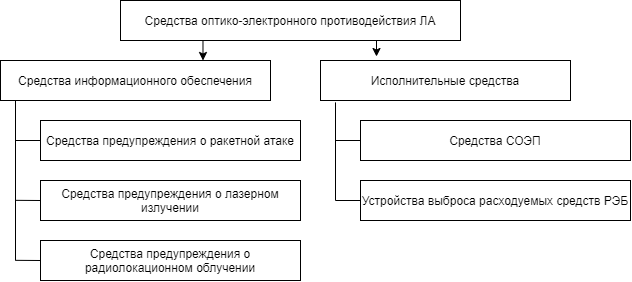
\includegraphics[width=0.8\linewidth]{pic1_2} 
	\caption{Классификация средств  \hyperref[acroSOEP]{СОЭП}  \hyperref[acroLA]{ЛА} \cite[]{ForeignMilitary}}
	\label{fig:classification}
\end{figure}

В качестве объекта исследования рассматривается автоматика системы средств СОЭП входящая в состав исполнительных средств. Ключевым элементом СОЭП является генератор пульсирующих инфракрасных помех представляет собой мощную инфракрасную лампу с вращающимся отражателем или способную изменять свою яркость с заданной частотой, в кожухе из прозрачного для инфракрасного излучения материала.

В качестве объекта наблюдения/противодействия будем считать ракету с инфракрасной головкой самонаведения (\hyperref[acroGSN]{ГСН}), относящуюся к самым универсальным управляемым средствам поражения воздушных целей. Принцип сканирования поля зрения \hyperref[acroGSN]{ГСН} показан на рисунке \ref{fig:rocketScanning}. 

\begin{figure}[ht]
	\centering
	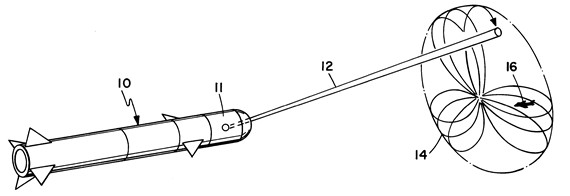
\includegraphics[width=0.6\linewidth]{p3} 
	\caption{Принцип сканирования головкой самонаведения ракеты}
	\label{fig:rocketScanning}
\end{figure}

На рисунке \ref{fig:rocketScanning}: 1 - Сканирующая система в составе \hyperref[acroGSN]{ГСН}, 2 - Сектор моментального поля зрения, 3 - Цель (летательный аппарат), 4 - Полное поле зрения \hyperref[acroGSN]{ГСН}.	
	
При генерировании пульсирующих инфракрасных помех с частотой, равной рабочей частоте внутренних элементов наведения, и мощностью, сопоставимой с естественным тепловым излучением защищаемой цели, в систему наведения ракеты вносится помеха, приводящая к отклонению ракеты от защищаемой цели. 
%Вероятность срыва атаки ракеты ПЗРК при использовании генераторов пульсирующих инфракрасных помех составляет от 0,5 до 0,7-0,8.

\subsection{ \hyperref[acroSOEP]{СОЭП} первого поколения}	

К ним относятся системы ненаправленной постановки помех. Такие системы не имеют системы наведения. Принцип действия такой станции основан на генерации всенаправленного модулированного помехового ИК-излучения со специальной структурой сигнала. К таким системам относятся \cite[]{SOEP_LIPA}: 1. «Липа» (РФ); 2. AN/ALQ-144 (США, смотри рисунок \ref{fig:alq}); 3. AN/ALQ-157 by BAE Systems, used for larger helicopters and aircraft; 4. AN/ALQ-212 by BAE Systems, currently fielded on U.S. Army CH-47 Chinook helicopters; 5. “Адрос КТ-01 АВ” (Украина); 6. “Квадрос-КМ-01 В” (Украина).

\begin{figure}[ht]
	\centering
	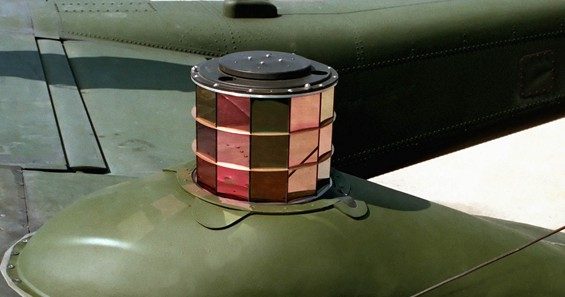
\includegraphics[width=0.4\linewidth]{p4} 
	\caption{ \hyperref[acroSOEP]{СОЭП} первого поколения}
	\label{fig:alq}
\end{figure}
На рисунке \ref{fig:alq} показана система постановки всенаправленных помех AN/ALQ-144 установленная на борту летательного аппарата. Устройство не имеет подвижных частей, ИК излучение от источника проходит через фильтр и распространяется в верхней полусфере.

 \hyperref[acroSOEP]{СОЭП} первого поколения обеспечивают защиту военной авиационной техники от ракетных комплексов с инфракрасными головками самонаведения (ИК \hyperref[acroGSN]{ГСН}) типа «Сайдуиндер», «Ред Ай», «Чапарэл», «Питон», «Стрела-2М», «Хунинь-5» и им подобных. 

\subsection{ \hyperref[acroSOEP]{СОЭП} второго поколения}	

К  системам второго поколения относятся системы с узконаправленным ОЭП (DIRCM) модулированным пучком помехового излучения. Примеры приведены на рисунке \ref{fig:p6-7}.

В состав комплекса входит станции предупреждения о ракетной атаке, имеющие ряд общих особенностей:
\begin{itemize}
	\item модульность конструкции, сравнительно малая масса (7-17 кг) и размеры;
	\item потребляемая мощность порядка 70-100 Вт;
	\item обнаружение атакующих ракет в секторах до 360° в азимутальной и до 180° в угломестной плоскости на дальности 3-10 км с угловым разрешением порядка 1° или меньше;
	\item в большинстве станций используются датчики, функционирующие в УФ-диапазоне ЭМВ.
\end{itemize}

Принцип работы  \hyperref[acroSOEP]{СОЭП} узконаправленным пучком основан на раннем обнаружении пуска ракеты, ее сопровождении и подавлении канала наведения с использованием узконаправленного потока модулированного ИК излучения. Работа средств направленного оптико-электронного противодействия ракетной атаке осуществляется в последовательности описанной на рисунке \ref{fig:p5}) \cite[]{ForeignMilitary}:

\begin{enumerate}
	\item Обнаружение атакующей ракеты средствами информационного обеспечения в спектральных диапазонах 0,01-0,4 мкм (УФ) и 4-14 мкм (ИК);
	\item Формирование ложного сигнала от цели; 
	\item Срыв наведения на цель; 
	\item Цель вне поля зрения \hyperref[acroGSN]{ГСН} ракеты; 
	\item Ракета не представляет угрозы для вертолета.	
\end{enumerate}

\begin{figure}[ht]
	\centering
	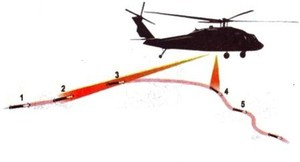
\includegraphics[width=0.5\linewidth]{p5} 
	\caption{Схема работы  \hyperref[acroSOEP]{СОЭП} при атаке ракетой с головкой самонаведения}
	\label{fig:p5}
\end{figure}

Использование нескольких излучателей, размещенных на  \hyperref[acroLA]{ЛА}, ЦСУ и оперативного перепрограммирования режимов работы значительно увеличивает вероятность противодействия угрозе ракетной атаки.

%\begin{figure}[ht]
%	\centering
%	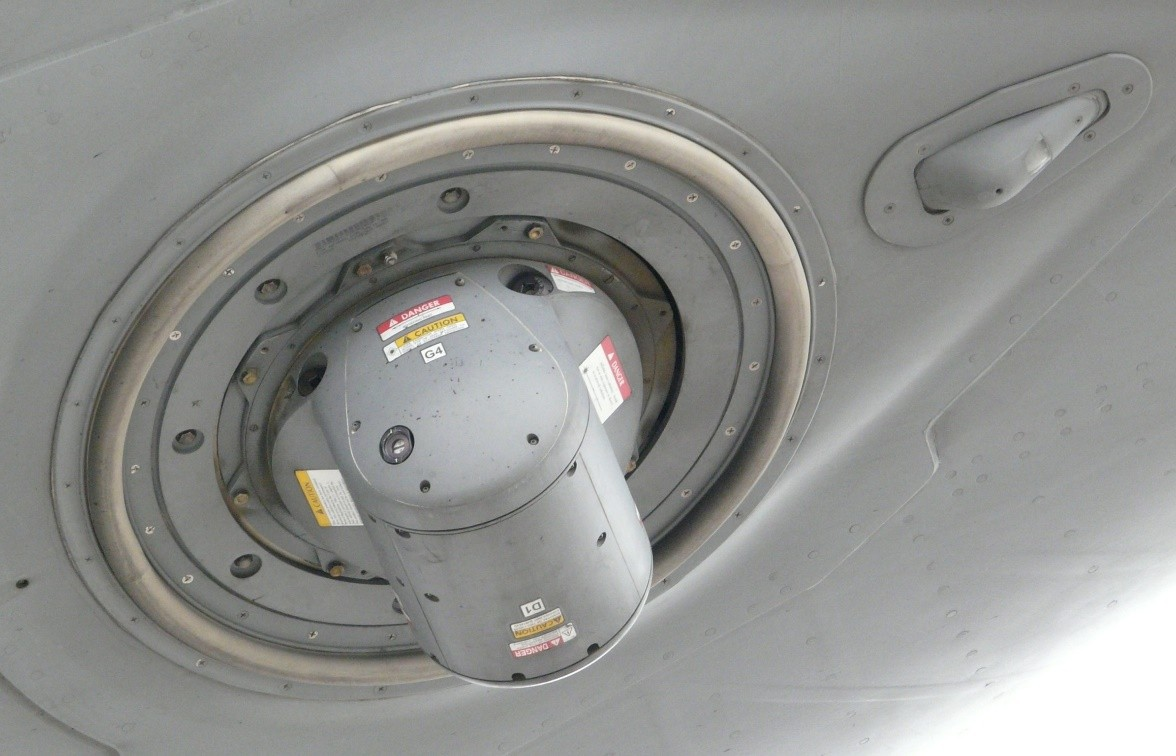
\includegraphics[width=0.5\linewidth]{p6} 
%	\caption{ \hyperref[acroSOEP]{СОЭП} пульсирующих инфракрасных помех}
%	\label{fig:p6}
%\end{figure}

\begin{figure}[ht]
	\begin{minipage}[b][][b]{0.49\linewidth}\centering
		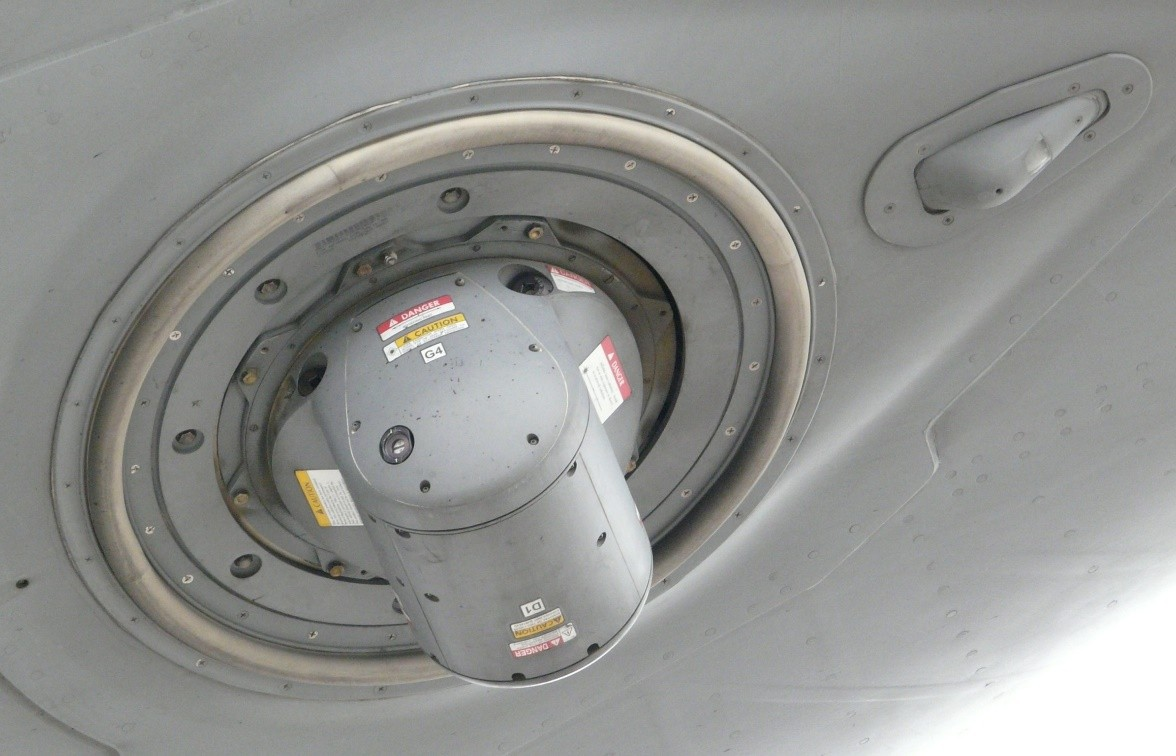
\includegraphics[width=0.8\linewidth]{p6} \\ а)
	\end{minipage}
	\hfill
	\begin{minipage}[b][][b]{0.49\linewidth}\centering
		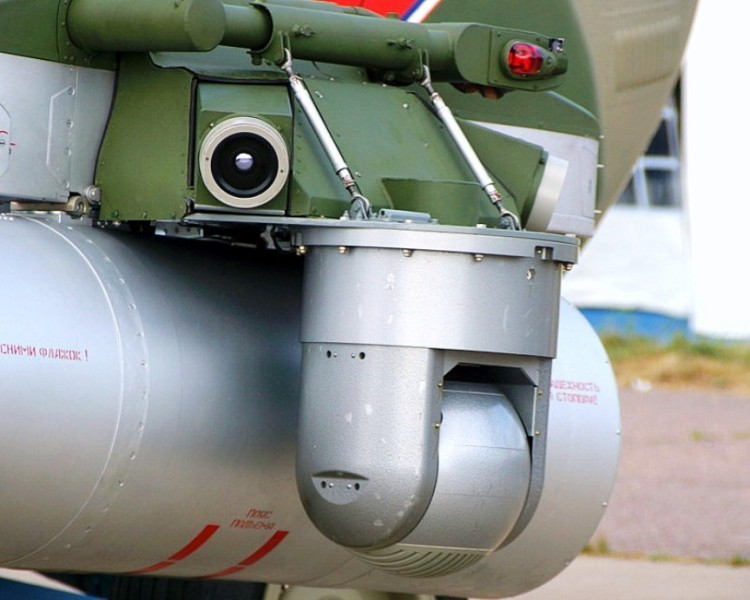
\includegraphics[width=0.7\linewidth]{p7} \\ б)
	\end{minipage}
	
	%\centering
	%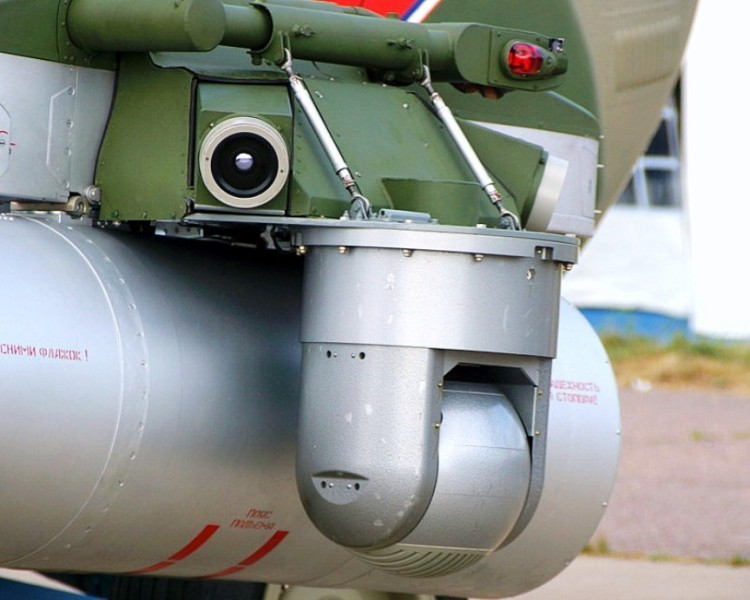
\includegraphics[width=0.5\linewidth]{p7} 
	\caption{а)\hyperref[acroSOEP]{СОЭП} пульсирующих инфракрасных помех; б)Станция Л370-5 и УФ пеленгатор пуска ракет Л370-5-02}
	\label{fig:p6-7}
\end{figure}

\hyperref[acroSOEP]{СОЭП} такого типа разработаны \cite[]{Infrared_countermeasure}:
\begin{itemize}
	\item Президент-С (рисунок \ref{fig:p6-7} б);
	\item Leonardo’s Miysis DIRCM (directed infrared countermeasure);
	\item AN/AAQ-24 (Northrop Grumman) AN/ALQ-132 (Sanders/BAE Systems);
	\item CAMPS (Saab Avitronics);
	\item CIRCM (Northrop Grumman) (рисунок \ref{fig:p6-7} а);
	\item Selex ES' Miysis System;
	\item "Сухогруз" (используется на Су-25T);
	\item KT-01 AVE, KT-02 ACE(Adron).		
\end{itemize}



\subsection{ \hyperref[acroSOEP]{СОЭП} третьего поколения}	
К  ним относятся лазерные системы защиты. Основными преимуществами таких систем являются независимость эффективности \hyperref[acroSOEP]{СОЭП} от принципа работы головок наведения ракет, их меньший вес и габариты по сравнению с комплексами второго поколения. Визуальный облик их показан на рисунке \ref{fig:p8-9}, принцип работы которых основан на взаимодействии лазерного излучения с веществом где возникает порог разрушения: физический (нарушается работоспособность изделия) и технический (происходят необратимые изменения оптических характеристик образца (пропускания, рассеяния, отражения) материала)\cite[]{manta}. 

%\textbf{Физическим} порогом разрушения материала называют такую плотность энергии или мощности (интенсивность) излучения, при которой происходят необратимые изменения оптических характеристик образца (пропускания, рассеяния, отражения) исследуемого материала. Изменение указанных характеристик является следствием образования разрушения, формирование которого сопровождается яркой вспышкой оптического излучения. 

\begin{figure}[ht]
	\begin{minipage}[b][][b]{0.49\linewidth}\centering
		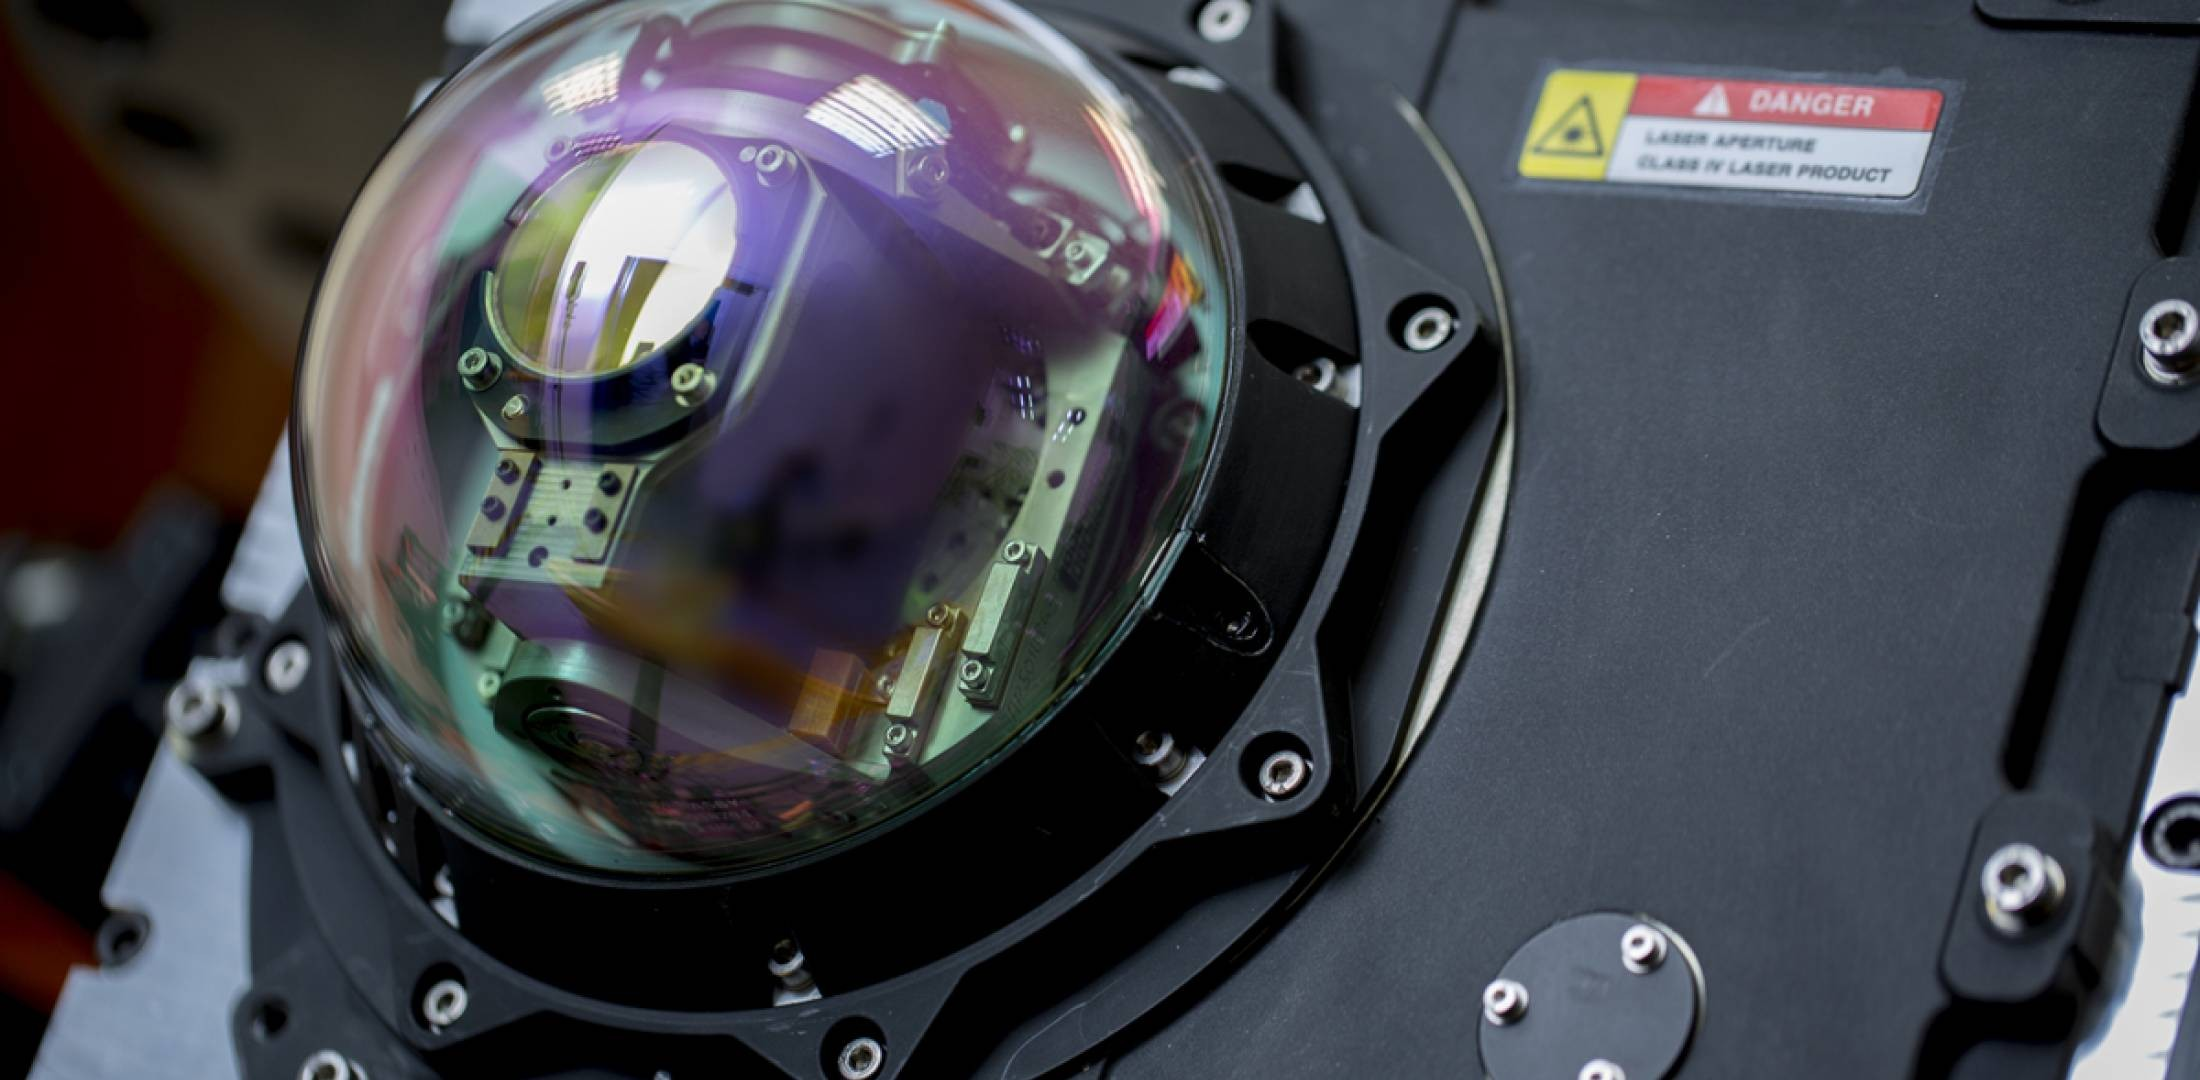
\includegraphics[width=0.8\linewidth]{p8} \\ а)
	\end{minipage}
	\hfill
	\begin{minipage}[b][][b]{0.49\linewidth}\centering
		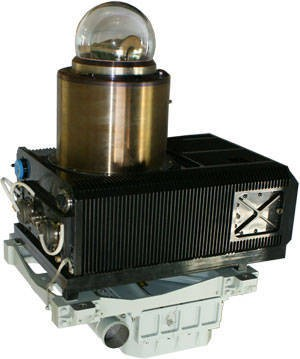
\includegraphics[width=0.5\linewidth]{p9} \\ б)
	\end{minipage}

	%\centering
	%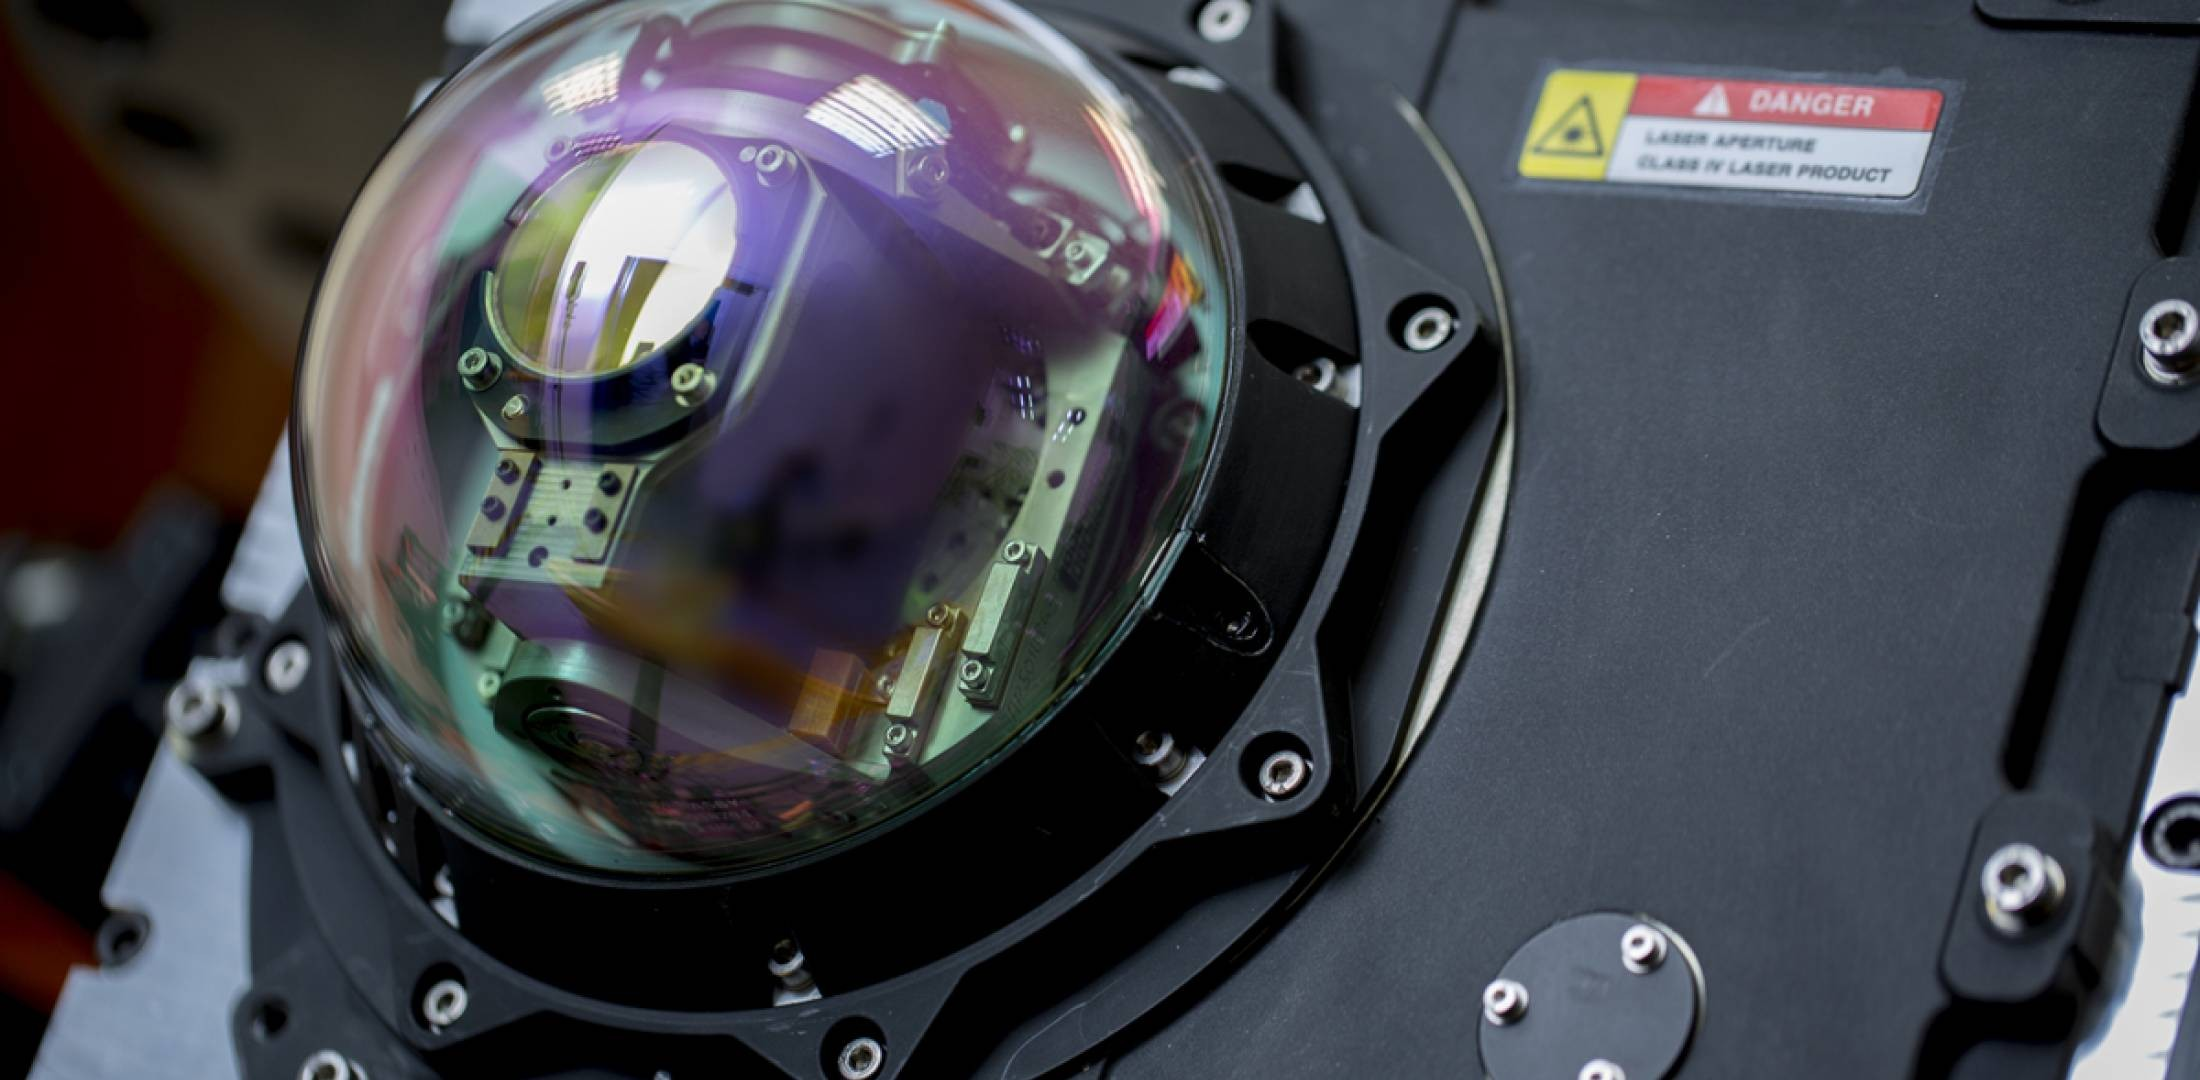
\includegraphics[width=0.7\linewidth]{p8} 
	\caption{а)Автоматическая бортовая лазерная станция постановки помех ALJS; б)Изделие Л370В28 (лазерная станция постановки помех)}
	\label{fig:p8-9}
\end{figure}

%\textbf{Техническим} порогом разрушения называют такую плотность энергии или мощности излучения, при которой нарушается работоспособность изделия, изготовленного из исследуемого материала, вследствие изменений его оптических характеристик, превышающих допустимые.

Одним из немногих примеров комплексов третьего поколения является система MANTA (Испания). Это автоматическая бортовая лазерная станция постановки помех ALJS \cite[]{manta}.
Ее работа основывается на использовании кодированного мультиспектрального излучения импульсно-периодического (HF/DF) лазера для создания помех в широком ИК-диапазоне.
Российский комплекс третьего поколения носит название Л370В28, его внешний вид показан на рисунке \ref{fig:p8-9} б. 

%\begin{figure}[ht]
%	\centering
%	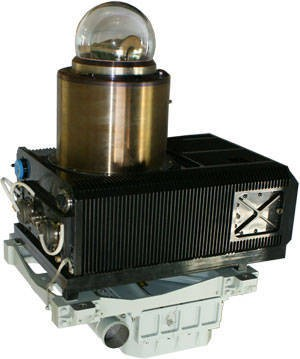
\includegraphics[width=0.3\linewidth]{p9} 
%	\caption{Изделие Л370В28 (лазерная станция постановки помех)}
%	\label{fig:p9}
%\end{figure}

Особенностями средств направленного ОЭП являются \cite[]{ForeignMilitary}:
\begin{itemize}
	\item высокий энергетический потенциал лазерного излучения;
	\item возможность функционального поражения приемных элементов ИК \hyperref[acroGSN]{ГСН}, а также поражения (ослепления) операторов комплексов вооружения и стрелков при наведении лазерного луча на источник угрозы по информации от средств обнаружения угрозы;
	\item обеспечение синхронизации со средствами обнаружения угрозы для получения информации о направлении на источник угрозы;
	\item необходимость целеуказания на источник угрозы с точностью до нескольких угловых минут;
	\item возможность функционирования в составе систем, включающих несколько станций ОЭП;
	\item возможность совместного функционирования с устройствами выброса расходуемых средств РЭБ.
\end{itemize}



\section{Элементная база для обеспечения обратной связи САУ \hyperref[acroEOS]{ОЭС}} \label{sec:ch1/sec3-}
Для системы автоматического управления наиболее важным элементом является обратная связь. В САУ  \hyperref[acroEOS]{ОЭС} рассматриваемого класса, в качестве датчиков обратной связи углового положения оптической оси используют следующие типы датчиков:

--- \textbf{СКВТ (Синусно-косинусный вращающийся трансформатор)} - являются двухобмоточными на статоре (в основном) или многополюсными электрическими машинами. По конструкции аналогичны синхронным электродвигателям с возбуждаемым переменным током ротора \cite[]{SKVT}. 
%В зависимости от угловой ориентации магнитного поля ротора относительно взаимно перпендикулярным по магнитному потоку обмоток статора в обмотках статора наводится ЭДС, амплитуда и фаза которых зависит от угла поворота ротора относительно статора. Эти электрические сигналы однозначно, в пределах одного оборота ротора, характеризуют угол поворота ротора \cite[]{SKVT}.
	
	\begin{figure}[ht]
		\centering
		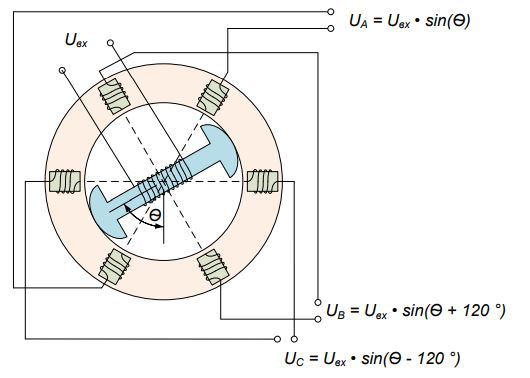
\includegraphics[width=0.5\linewidth]{SKVT} 
		\caption{Принципиальная электромеханическая схема СКВТ \cite[]{1310HM025}}
		\label{fig:SKVT}
	\end{figure}
	
--- \textbf{Датчик Холла совместно с оптопарой в качестве датчика нуля}. Магнитный датчик на эффекте Холла регистрируют прохождение магнитных полюсов вращающегося магнитного элемента непосредственно вблизи чувствительного элемента, преобразуя эти данные в соответствующий цифровой код или сигнал \cite[]{Encoder}.
	
--- \textbf{Энкодер}. Оптические датчики углового положения (\hyperref[acroDUP]{ДУП}) имеют жёстко закреплённый на валу стеклянный диск с оптическим растром. При вращении вала растр перемещается относительно неподвижного растра, при этом модулируется световой поток, принимаемый фотодатчиком. Абсолютные оптические датчики угла — это датчики угла поворота, в которых каждому положению вала соответствует цифровой выходной код, который наряду с числом оборотов является основным рабочим параметром датчика. Абсолютные оптические \hyperref[acroDUP]{ДУПы}, так же как и накапливающие, считывают и фиксируют параметры вращения оптического диска \cite[]{Encoder}.

С ростом технологичности электронной компонентной базы и появлением возможности обработки изображения в реальном времени для систем смотрящего типа обратную связь можно обеспечить обработкой информации с фотоприемника. Для этого используют:

--- \textbf{Одноэлементные фотоприемники с применением механических модуляторов}. Для определения координат используется амплитудно-фазовый метод. С помощью анализатора в виде диска с переменной прозрачностью, изменяющейся по закону светового клина \cite[]{bibook1}. Схема работы показана на рисунке~\ref{fig:p10}.
	
	\begin{figure}[ht]
		\centering
		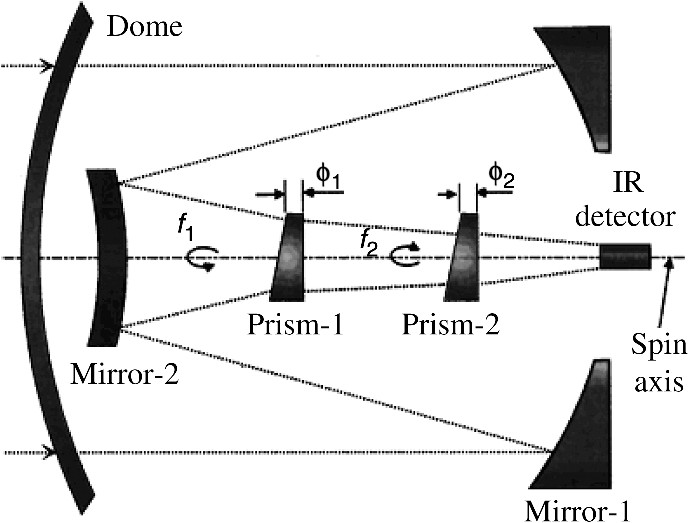
\includegraphics[width=0.5\linewidth]{p10} 
		\caption{Оптическая схема одноэлементной сканирующей \hyperref[acroGSN]{ГСН} }
		\label{fig:p10}
	\end{figure}

--- \textbf{Позиционно чувствительные фотоприемники}. Приемное устройство представляет собой четырехквадратный фотодиод. Определение отклонения изображения объекта происходит путем вычисления разницы напряжений между элементами. На рисуноке~\ref{fig:4px} показана конструкция фотоприемника.	
	\begin{figure}[ht]
		\centering
		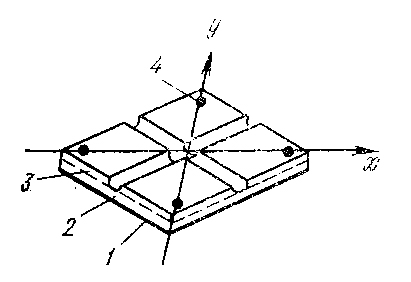
\includegraphics[width=0.4\linewidth]{4px} 
		\caption{Позиционно-чувствительный фотодиод. 1 - кристаллодержатель; 2 - \textit{n}-область; 3 - \textit{p}-область; 4 - контакт.}
		\label{fig:4px}
	\end{figure}
	


--- \textbf{Многоэлементные матричные фотоприемники}. ПЗС-матрица — специализированная аналоговая интегральная микросхема, состоящая из светочувствительных фотодиодов, выполненная на основе кремния, использующая технологию ПЗС — приборов с зарядовой связью. Принципиальная схема показана на рисунке \ref{fig:EMCCD2_color_en}\cite[]{CCD2}.
	
ПЗС-матрицы выпускаются и широко используются компаниями Nikon, Canon, Sony, Fujitsu, Kodak, Matsushita, Philips и многими другими. В России ПЗС-матрицы сегодня разрабатывают и выпускают: ОАО "ЦНИИ Электрон" и его дочернее предприятие ЗАО "НПП Элар", а также ОАО "НПП Пульсар" (г. Москва)\cite[]{CCD}.
	
Наиболее приоритетный тип фотоприёмных устройств на данное время. Повсеместно используется в гражданской продукции, нам интересны ПЗС матрицы ИК спектра.
	
	\begin{figure}[ht]
		\centering
		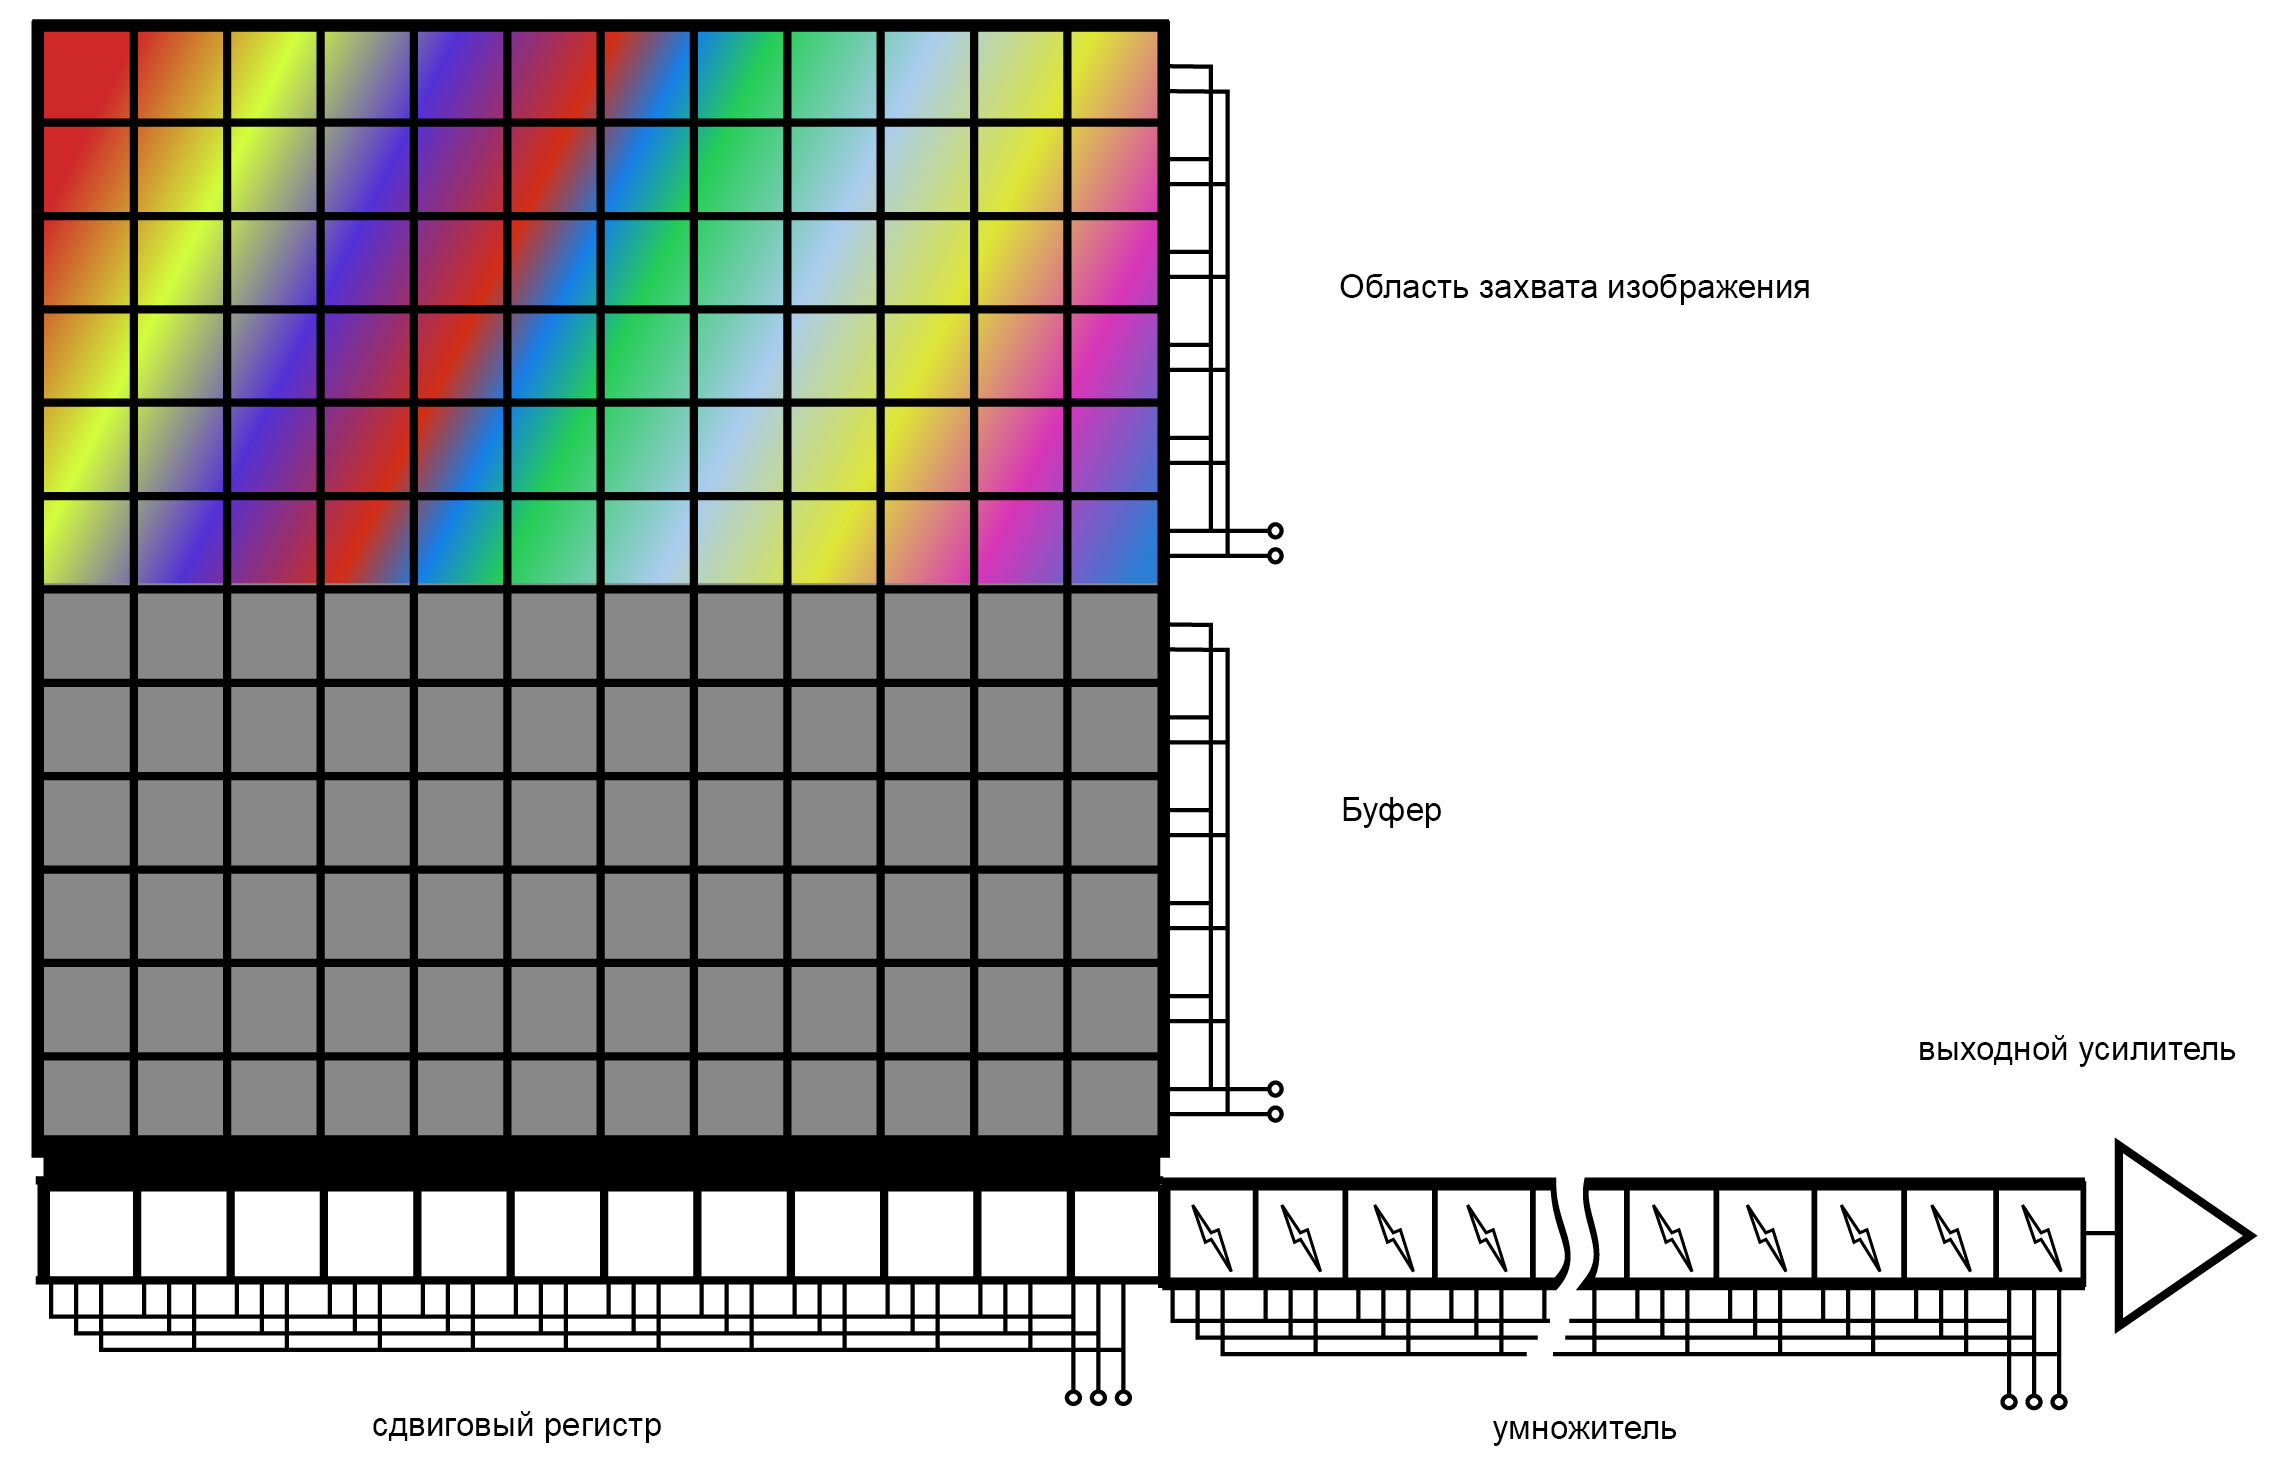
\includegraphics[width=0.4\linewidth]{EMCCD2_color_en} 
		\caption{Схема позиционно-чувствительного фотодиода}
		\label{fig:EMCCD2_color_en}
	\end{figure}
	

\section{Математические модели, динамика и управление, синтез и компьютерное моделирование САУ бортовых ОЭС} \label{sec:ch1/modeling}

Большое внимание в последние годы в публикациях уделяется динамике, управлению и стабилизации изображения бортовых ОЭС и комплексов, как одному из факторов, влияющих на качество изображения. Вопросы разработки САУ бортовых ОЭС посвящены работы []. В них обсуждается разработка расчетных и математических моделей, декомпозиция и идентификация многомерных систем, синтез и компьютерное моделирование, в том числе макетирование нелинейных систем. Первые публикации, посвященные решению указанных выше вопросов появились в трудах международных симпозиумов по автоматическому управлению (1975,1976 г.),позднее в трудах международных Чтаевских конференций, в трудах КАИ, в журналах: "Оптический журнал", "Гироскопия и навигация", "Авиационная техника", "Вестник КГТУ им. Туполева".

Разработка адекватных математических моделей, методики синтеза алгоритмов и исследование динамики управления бортовыми ОЭС раскрывается в работах Матросова В.М.[], Васильева С.Н., Дегтярева Г.Л., Стрежнева В.А.[], Землякова В.А., Маливанова М.Н., Кренева В.А., Карпова А.И., Николаева Р.П., Маханько А.В.

В связи с изменениями параметров среды, в которой функционирует ОЭС, широко используется метод компьютерного моделирования, применение которого для разработки и исследования ОЭС применяется в работах Якушенкова Ю.Г.,Торанено И.П., Иванова В.П., Балоева В.А.,Овсянникова В.А., Филипова В.П., Яцыка В.С., Маливанова Н.Н., Кренева В.А., Карпова А.И., Михалицына А.В., Молина Д.А.

Следует отметить используемые для конкретного применения компьютерные модели (КМ): CASiEL (Израиль)[], FLIR, FCSS, COMOC, КМ ОЭС, Htm2008 НПО ГИПО, где используются моделирование характеристик ОЭС на основе применения оптической передаточной функции (ОПФ). Применение КМ ОЭС является универсальным средством для анализа  и синтеза сложных ОЭС, удобным методом исследования их эффективности при широком изменении параметров.

%Однако применение указанных в этом разделе обзора  математических моделей и методов разработки и исследования динамики не представляется возможным из-за специфики излучающих ОЭС, так как в каждом конкретном случае можно использовать только "идею" разработки.

\section{Выводы по главе} \label{sec:ch1/sec4-}

\newcounter{c1}

\stepcounter{c1}
\arabic{c1}. Оптико-электронные системы можно разделить на группы:
%\begin{itemize}
--- \textbf{Смотрящего типа}. Характерными требованиями является точность позиционирования и стабилизации оси визирования. На настоящий момент серийно производимые приборы достигают точности 10 угловых минут.
	
--- \textbf{Излучающие}. Характерным требованием является время и скорость наведения. На настоящий момент серийно производимые приборы обеспечивают угловые скорости 700 градусов за секунду, при точности стабилизации порядка 5 угловых градусов.
	
--- \textbf{Комбинированные}. Характерным требованием является скорость наведения и точность позиционирования.
	
%\end{itemize}

Ниже приведем основные характеристики указанных бортовых оптико-электронных систем: точность позиционирования, скорость наведения, разрешение , спектральный диапазон, частота опроса фотоприемника, поле зрения.

\stepcounter{c1}
\arabic{c1}. Для каждого поколения  \hyperref[acroSOEP]{СОЭП} имеем свои особенности. Для \textbf{первого поколения}: одновременное покрытие всей рабочей полусферы, простота конструкции, малая мощность излучения, малая глубина модуляции, сильная привязка к типу подавляемой ракеты; для \textbf{второго поколения}: большая мощность излучения, возможность генерации различного типа модуляции, более сложная конструкция, малая точность наведения, большая масса по сравнению с I поколением; для \textbf{третьего поколения}: работоспособность не зависит от типа подавляемой ракеты, использование когерентного излучения, малая ширина спектра излучения, большая масса по сравнению с I поколением, большая точность наведения.

Основными направлениями развития подобных средств противодействия являются: повышение быстродействия, использование лазеров, перестраиваемых в широком диапазоне длин волн, уменьшение размеров и массы, увеличение энергетического потенциала лазерного излучения, унификация оборудования (возможность использования на любом типе носителя, возможность согласованного функционирования с различными типами средств ИО и исполнительных средств РЭБ), модульность конструкции и открытая архитектура.
%Данный обзор заключает в себе общую информацию о  \hyperref[acroSOEP]{СОЭП}. 
%В главах \ref{ch:ch3}, \ref{ch:ch4} (\nameref{ch:ch3}, \nameref{ch:ch4}) проводятся расчеты позволяющие повысить быстродействие, точность, уменьшить массу средств противодействия.

\stepcounter{c1}
\arabic{c1}. Основная элементная база бортовых оптико-электронных систем можно объединить:
--- \textbf{по управляющей координате}. При использовании 16 разрядного датчика можно достич точности определения координаты порядка 20 угловых секунд, в реальном приборе точность отработки управляющего воздействия ограничивается точностью исполнительного устройства.
	
	\begin{itemize}
		\item СКВТ (Синусно-косинусный вращающийся трансформатор)
		\item Датчик ХОЛЛА + датчик нуля (оптопара)
		\item Энкодер
	\end{itemize}
		
--- \textbf{по сигналу рассогласования с фотоприемника}. Широко применяются: одноэлементные фотоприемники с применением механических модуляторов, позиционно чувстительные фотоприемники, многоэлементные матричные фотоприемники. Например, фотоприемник с частотой опроса 400 Гц и разрешением 512х512 пикселей можно достичь точность сопровождения цели порядка 10 угловых секунд.

\begin{comment}
Проведена оценка точности при использовании различных датчиков.Исследование влияния точности и принципа работы датчика проводится в главе \ref{ch:ch5} (\nameref{ch:ch5}).
\end{comment}

\stepcounter{c1}
\arabic{c1}. Кроме оптических характеристик на качество ОЭП в значительной степени влияет время сканирования определенной части пространства, время выхода на заданное целеуказание и точность сопровождения цели. Оно осуществляется двумя способами: путем перемещения всего устройства информационных каналов или управления положением отдельных оптических элементов (зеркал, призм). Применение второго способа обеспечивает высокие динамические и точностные характеристики. 

По этим причинам и возникает актуальная задача увеличения точности наведения и удержания цели, что неизбежно ведет за собой необходимость разработки \hyperref[acroEOS]{ОЭС}, как объекта управления, алгоритмов управления, математической модели, исследование систем управления, затрагивающими динамическую составляющую, как носителя, так и самого прибора. Кроме того, более точная математическая модель позволяет в дальнейшем решать задачу рационального выбора характеристик прибора по требуемым критериям.
 
Важным этапом разработки любого изделия является создание математической модели, макетирование и моделирование динамики. Распространенной проблемой при разработке изделий является отсутствие универсальной методики разработки и исследования динамики систем управления бортовыми оптико-электронными приборами. Применение информационных технологий таких как CAD/CAM средства проектирования, средства математического моделирования (MATHCAD, MatLAB, SolidWorks), средства контроля версий позволяют минимизировать человеческий фактор (Git), а следование методике разработки позволяет обеспечить выполнение изначальных требований к проектируемому изделию. 
%Решение вопросов такого характера обсуждается в главе \ref{ch:ch2} (\nameref{ch:ch2}).

Обобщая вышеизложенное о смотрящих БОЭП и  СОЭП, работающие в соответствующих режимах наведения, стабилизации и слежения при действии возмущений и наличии соответствующих ограничений, предметом данной работы целесообразным является решение задачи синтеза, моделирования и исследования динамики САУ БОЭП наблюдения и противодействия, конструктивно объединенные в единый прибор, управляемый по двум осям, функциональная схема которого приведена на рисунке \ref{fig:functional_scheme}.


\begin{figure}[ht]
	\centering
	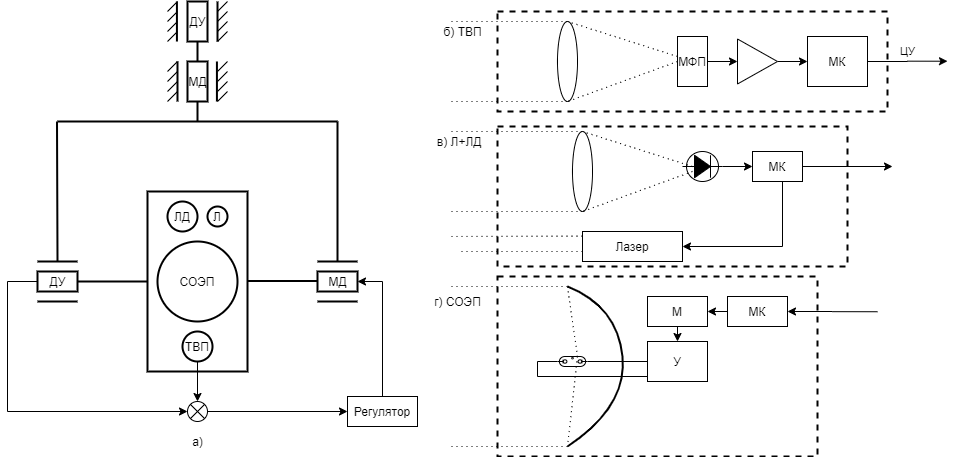
\includegraphics[width=0.9\linewidth]{func_scheme} 
	\caption{Функциональная схема САУ БОЭП наблюдения и противодействия}
	\label{fig:functional_scheme}
\end{figure}

\begin{itemize}
	\item 1 - объектив,
	\item 2 - узел излучателя,
	\item 3 - внутренний узел управления по углу места,
	\item 4 - внешний узел управления по азимуту,
	\item 5 - корпус прибора,
	\item 6 - защитное стекло,
	\item 7 - система охлаждения излучателя,
	\item 8 - узел моментного двигателя по азимуту,
	\item 9 - узел моментного двигателя по углу места.
\end{itemize}

Для выполнения поставленной цели необходимо решить следующие задачи:

\begin{enumerate}
	\item Разработка методики синтеза систем наведения и стабилизации оси визирования (Глава \ref{ch:ch2});
	\item Разработка математической модели ОЭС, как объекта управления, с учетом конструктивных особенностей, условий эксплуатации и имеющихся ограничений (Глава \ref{ch:ch3});
	\item Оценка допуска на точность стабилизации;
	\item Декомпозиция двухсвязной САУ с нелинейными элементами в составе ОУ;
	\item Идентификация;
	\item Синтез алгоритмов наведения на заданные углы в требуемых пределах за минимальное время и стабилизации оси визирования с точностью, обеспечивающей выполнение поставленной задачи (Глава \ref{ch:ch4});
	\item Разработка компьютерной имитационной модели системы наведения и стабилизации в пространстве (Глава \ref{ch:ch5});
	\item Исследование динамики управления БОЭС в режимах наведения и стабилизации с учетом действующих возмущений, нелинейностей и ограничений;
\end{enumerate}

\clearpage